% !TeX program = xelatex
% XA-202609 竞赛交付文稿；干净编译：XeLaTeX -> BibTeX -> XeLaTeX -> XeLaTeX
\documentclass[UTF8,a4paper,12pt]{ctexart}

\usepackage[margin=2.5cm]{geometry}
\usepackage{graphicx}
\usepackage{booktabs}
\usepackage{tabularx}
\usepackage{array}
\usepackage{placeins}
\usepackage{float}
\usepackage{caption}
\usepackage{amsmath}
\usepackage{xcolor}
\usepackage{listings}
\usepackage[numbers,sort&compress]{natbib}
\usepackage[colorlinks=true,linkcolor=blue!50!black,citecolor=blue!50!black,urlcolor=blue!50!black]{hyperref}

\graphicspath{{figures/}}
\captionsetup{font=small,labelfont=bf}
\setlength{\emergencystretch}{2em}
\newcolumntype{Y}{>{\raggedright\arraybackslash}X}
\newcommand{\xor}{\ensuremath{\oplus}}
\newcommand{\method}{Resource-NMCTS}
% AUTO-GENERATED by analysis/build_final_primary20_report.py; do not edit.
\newcommand{\FinalAnalysisID}{xa202609-primary20-836553591061}
\newcommand{\FinalDatabaseSHA}{8cc494ed4506f245d29bebbb8e328a991558c0d4f67d0d2b9244bab2bad77be7}
\newcommand{\FinalAnalysisContractSHA}{aebc28f87703717d4dc6c5b48b8421e8c1c7b9d5b801b53ce46d165671d4bf48}
\newcommand{\FinalPlannedCells}{360}
\newcommand{\FinalVerifiedCells}{360}
\newcommand{\FinalMissingCells}{0}
\newcommand{\FinalCoveragePct}{100.0}
\newcommand{\DirectAnfLogicTN}{20}
\newcommand{\DirectAnfLogicTPct}{51.5}
\newcommand{\DirectAnfLogicTPctLow}{39.1}
\newcommand{\DirectAnfLogicTPctHigh}{63.0}
\newcommand{\DirectAnfLogicTHolmP}{0.0005815}
\newcommand{\DirectAnfLogicTWTL}{17/3/0}
\newcommand{\DirectAnfLogicTStrict}{yes}
\newcommand{\DirectAnfLogicCnotN}{20}
\newcommand{\DirectAnfLogicCnotPct}{16.6}
\newcommand{\DirectAnfLogicCnotPctLow}{4.9}
\newcommand{\DirectAnfLogicCnotPctHigh}{23.7}
\newcommand{\DirectAnfLogicCnotHolmP}{0.001179}
\newcommand{\DirectAnfLogicCnotWTL}{14/3/3}
\newcommand{\DirectAnfLogicCnotStrict}{yes}
\newcommand{\DirectAnfNativeTwoQN}{20}
\newcommand{\DirectAnfNativeTwoQPct}{42.0}
\newcommand{\DirectAnfNativeTwoQPctLow}{7.5}
\newcommand{\DirectAnfNativeTwoQPctHigh}{67.5}
\newcommand{\DirectAnfNativeTwoQHolmP}{0.001836}
\newcommand{\DirectAnfNativeTwoQWTL}{14/3/3}
\newcommand{\DirectAnfNativeTwoQStrict}{yes}
\newcommand{\DirectAnfMappedDepthN}{20}
\newcommand{\DirectAnfMappedDepthPct}{45.2}
\newcommand{\DirectAnfMappedDepthPctLow}{6.1}
\newcommand{\DirectAnfMappedDepthPctHigh}{71.7}
\newcommand{\DirectAnfMappedDepthHolmP}{0.001836}
\newcommand{\DirectAnfMappedDepthWTL}{14/3/3}
\newcommand{\DirectAnfMappedDepthStrict}{yes}
\newcommand{\GreedyFactorLogicTN}{20}
\newcommand{\GreedyFactorLogicTPct}{23.6}
\newcommand{\GreedyFactorLogicTPctLow}{17.3}
\newcommand{\GreedyFactorLogicTPctHigh}{34.4}
\newcommand{\GreedyFactorLogicTHolmP}{0.001264}
\newcommand{\GreedyFactorLogicTWTL}{15/5/0}
\newcommand{\GreedyFactorLogicTStrict}{yes}
\newcommand{\GreedyFactorLogicCnotN}{20}
\newcommand{\GreedyFactorLogicCnotPct}{18.1}
\newcommand{\GreedyFactorLogicCnotPctLow}{0.0}
\newcommand{\GreedyFactorLogicCnotPctHigh}{23.0}
\newcommand{\GreedyFactorLogicCnotHolmP}{0.002367}
\newcommand{\GreedyFactorLogicCnotWTL}{12/5/3}
\newcommand{\GreedyFactorLogicCnotStrict}{no}
\newcommand{\GreedyFactorNativeTwoQN}{20}
\newcommand{\GreedyFactorNativeTwoQPct}{16.1}
\newcommand{\GreedyFactorNativeTwoQPctLow}{0.0}
\newcommand{\GreedyFactorNativeTwoQPctHigh}{22.8}
\newcommand{\GreedyFactorNativeTwoQHolmP}{0.002367}
\newcommand{\GreedyFactorNativeTwoQWTL}{12/5/3}
\newcommand{\GreedyFactorNativeTwoQStrict}{no}
\newcommand{\GreedyFactorMappedDepthN}{20}
\newcommand{\GreedyFactorMappedDepthPct}{16.9}
\newcommand{\GreedyFactorMappedDepthPctLow}{0.0}
\newcommand{\GreedyFactorMappedDepthPctHigh}{25.1}
\newcommand{\GreedyFactorMappedDepthHolmP}{0.001709}
\newcommand{\GreedyFactorMappedDepthWTL}{12/5/3}
\newcommand{\GreedyFactorMappedDepthStrict}{no}
\newcommand{\MctsFactorLogicTN}{20}
\newcommand{\MctsFactorLogicTPct}{23.6}
\newcommand{\MctsFactorLogicTPctLow}{15.5}
\newcommand{\MctsFactorLogicTPctHigh}{34.4}
\newcommand{\MctsFactorLogicTHolmP}{0.001264}
\newcommand{\MctsFactorLogicTWTL}{15/5/0}
\newcommand{\MctsFactorLogicTStrict}{yes}
\newcommand{\MctsFactorLogicCnotN}{20}
\newcommand{\MctsFactorLogicCnotPct}{19.6}
\newcommand{\MctsFactorLogicCnotPctLow}{0.0}
\newcommand{\MctsFactorLogicCnotPctHigh}{22.8}
\newcommand{\MctsFactorLogicCnotHolmP}{0.002367}
\newcommand{\MctsFactorLogicCnotWTL}{12/5/3}
\newcommand{\MctsFactorLogicCnotStrict}{no}
\newcommand{\MctsFactorNativeTwoQN}{20}
\newcommand{\MctsFactorNativeTwoQPct}{12.8}
\newcommand{\MctsFactorNativeTwoQPctLow}{0.0}
\newcommand{\MctsFactorNativeTwoQPctHigh}{22.8}
\newcommand{\MctsFactorNativeTwoQHolmP}{0.002367}
\newcommand{\MctsFactorNativeTwoQWTL}{12/5/3}
\newcommand{\MctsFactorNativeTwoQStrict}{no}
\newcommand{\MctsFactorMappedDepthN}{20}
\newcommand{\MctsFactorMappedDepthPct}{10.3}
\newcommand{\MctsFactorMappedDepthPctLow}{0.0}
\newcommand{\MctsFactorMappedDepthPctHigh}{25.1}
\newcommand{\MctsFactorMappedDepthHolmP}{0.001709}
\newcommand{\MctsFactorMappedDepthWTL}{12/5/3}
\newcommand{\MctsFactorMappedDepthStrict}{no}
\newcommand{\SshrHLogicTN}{20}
\newcommand{\SshrHLogicTPct}{10.0}
\newcommand{\SshrHLogicTPctLow}{-5.3}
\newcommand{\SshrHLogicTPctHigh}{29.2}
\newcommand{\SshrHLogicTHolmP}{0.7758}
\newcommand{\SshrHLogicTWTL}{10/4/6}
\newcommand{\SshrHLogicTStrict}{no}
\newcommand{\SshrHLogicCnotN}{20}
\newcommand{\SshrHLogicCnotPct}{-28.0}
\newcommand{\SshrHLogicCnotPctLow}{-54.5}
\newcommand{\SshrHLogicCnotPctHigh}{0.0}
\newcommand{\SshrHLogicCnotHolmP}{0.1871}
\newcommand{\SshrHLogicCnotWTL}{5/2/13}
\newcommand{\SshrHLogicCnotStrict}{no}
\newcommand{\SshrHNativeTwoQN}{20}
\newcommand{\SshrHNativeTwoQPct}{30.6}
\newcommand{\SshrHNativeTwoQPctLow}{3.0}
\newcommand{\SshrHNativeTwoQPctHigh}{40.2}
\newcommand{\SshrHNativeTwoQHolmP}{0.002579}
\newcommand{\SshrHNativeTwoQWTL}{14/2/4}
\newcommand{\SshrHNativeTwoQStrict}{yes}
\newcommand{\SshrHMappedDepthN}{20}
\newcommand{\SshrHMappedDepthPct}{38.3}
\newcommand{\SshrHMappedDepthPctLow}{-0.9}
\newcommand{\SshrHMappedDepthPctHigh}{47.7}
\newcommand{\SshrHMappedDepthHolmP}{0.002579}
\newcommand{\SshrHMappedDepthWTL}{13/1/6}
\newcommand{\SshrHMappedDepthStrict}{no}
\newcommand{\SshrBeamLogicTN}{20}
\newcommand{\SshrBeamLogicTPct}{40.9}
\newcommand{\SshrBeamLogicTPctLow}{21.2}
\newcommand{\SshrBeamLogicTPctHigh}{50.0}
\newcommand{\SshrBeamLogicTHolmP}{0.03901}
\newcommand{\SshrBeamLogicTWTL}{17/1/2}
\newcommand{\SshrBeamLogicTStrict}{yes}
\newcommand{\SshrBeamLogicCnotN}{20}
\newcommand{\SshrBeamLogicCnotPct}{-7.1}
\newcommand{\SshrBeamLogicCnotPctLow}{-39.8}
\newcommand{\SshrBeamLogicCnotPctHigh}{12.1}
\newcommand{\SshrBeamLogicCnotHolmP}{0.3544}
\newcommand{\SshrBeamLogicCnotWTL}{8/1/11}
\newcommand{\SshrBeamLogicCnotStrict}{no}
\newcommand{\SshrBeamNativeTwoQN}{20}
\newcommand{\SshrBeamNativeTwoQPct}{45.3}
\newcommand{\SshrBeamNativeTwoQPctLow}{34.1}
\newcommand{\SshrBeamNativeTwoQPctHigh}{50.5}
\newcommand{\SshrBeamNativeTwoQHolmP}{0.0007367}
\newcommand{\SshrBeamNativeTwoQWTL}{17/1/2}
\newcommand{\SshrBeamNativeTwoQStrict}{yes}
\newcommand{\SshrBeamMappedDepthN}{20}
\newcommand{\SshrBeamMappedDepthPct}{51.8}
\newcommand{\SshrBeamMappedDepthPctLow}{40.6}
\newcommand{\SshrBeamMappedDepthPctHigh}{55.7}
\newcommand{\SshrBeamMappedDepthHolmP}{0.0007367}
\newcommand{\SshrBeamMappedDepthWTL}{17/1/2}
\newcommand{\SshrBeamMappedDepthStrict}{yes}


\lstset{
  basicstyle=\ttfamily\footnotesize,
  columns=fullflexible,
  keepspaces=true,
  frame=single,
  breaklines=true,
  breakatwhitespace=true,
  language=bash
}

\title{\method{}：面向 bit-flip Boolean Oracle 的\\
可验证资源感知组合综合与硬件映射\\[0.5em]
{\large AI 辅助量子编译的 XA-202609 竞赛级实现}}
\author{XA-202609 参赛团队}
\date{2026 年 7 月}

\begin{document}

\maketitle

\begin{abstract}
量子布尔函数 Oracle 是 Grover 型搜索与量子密码分析中的基础编译对象，但从真值表到可执行线路之间同时存在逻辑表示、资源权衡、辅助比特管理和硬件拓扑约束。本文实现 \method{}，将 bit-flip Boolean Oracle 综合写成 ANF/FPRM 项集合上的资源约束搜索，并以可验证的候选组合机制在 Direct-ANF、因子贪心、启发式 MCTS、仿射/FPRM 变换和可选的监督动作评分器之间选择线路。公共 artifact API 保存真实 X/CNOT/MCT 门序列；Qiskit Target、HLS 与 SABRE 完成无校准 synthetic Target 映射；逻辑穷举和映射后全部 $(x,y)$ 基态验证共同检查功能、辅助位、泄漏与输入相关相位。冻结主分析覆盖 20 个函数、6 个方法和 3 个综合 seed：360 个计划单元全部完成双层精确验证。以独立 Boolean 函数为推断单位，相对 Direct-ANF，\method{} 的逻辑 T、逻辑 CNOT、native-2Q 和 mapped depth 中位相对改善分别为 $51.5\%$、$16.6\%$、$42.0\%$ 和 $45.2\%$，四项 95\% bootstrap 区间均严格位于有利方向，分族 Holm 校正 $p_{\mathrm H}\leq0.00184$。相对 Greedy/MCTS，严格支持集中在逻辑 T；相对 SSHR-H，严格支持 native-2Q；相对 SSHR-Beam 的 20 个完整函数，严格支持逻辑 T、native-2Q 和 mapped depth，而 CNOT 不占优。监督评分器的独立 clean pilot 主要为平局，完整 60 个 \method{} 单元中 54 个选择确定性分支，因此上述组合收益不归因于 learned prior，也不外推为真实硬件保真度收益。
\end{abstract}

\noindent\textbf{关键词：}量子编译；bit-flip Boolean Oracle；资源感知综合；蒙特卡洛树搜索；学习先验；硬件映射

\section{题意、任务与证据边界}

\subsection{榜题定位}

XA-202609“量子+AI 双向赋能的研究与应用探索”包含“AI 驱动的量子编译与线路优化”方向。本作品聚焦其中可精确验证的一类任务：给定 $n$ 输入 Boolean 函数 $f$，生成实现
\begin{equation}
  |x\rangle|y\rangle \longmapsto |x\rangle|y\xor f(x)\rangle
  \label{eq:oracle}
\end{equation}
的 bit-flip Oracle，并在统一成本、辅助比特和拓扑约束下比较候选线路。核心引擎不处理任意 unitary，也没有独立的高精度 Rz 或相位 Oracle 综合后端。

\subsection{双向赋能的实际含义}

\begin{itemize}
  \item \textbf{AI 辅助量子编译：}监督训练的动作评分器可作为 MCTS 候选排序先验；它与启发式、uniform 和固定 seed 随机先验在相同预算下消融。AI 不承担线路正确性判定。
  \item \textbf{量子问题为 AI 提供可审计基准：}Oracle 综合具有离散动作、精确目标函数和可穷举验证的小规模实例，可用于检验学习引导搜索何时有用、何时退化。这是结构化 benchmark 价值，不等同于已经用量子计算加速了 AI。
  \item \textbf{当前闭环：}系统已完成“Boolean 函数输入 $\to$ 逻辑综合 $\to$ synthetic Target 映射 $\to$ 本地无噪声精确验证 $\to$ DuckDB 归档”。真实芯片、校准噪声和保真度评测属于后续扩展。
\end{itemize}

\section{系统方案}

图~\ref{fig:arch} 给出从输入到可审计交付的完整数据流。系统把“产生候选”“选择候选”“验证语义”和“统计归档”分开，使学习模块的影响可被替换和消融，也使线路图、资源表与实验数据库共享同一门序列来源。

\begin{figure}[tbp]
  \centering
  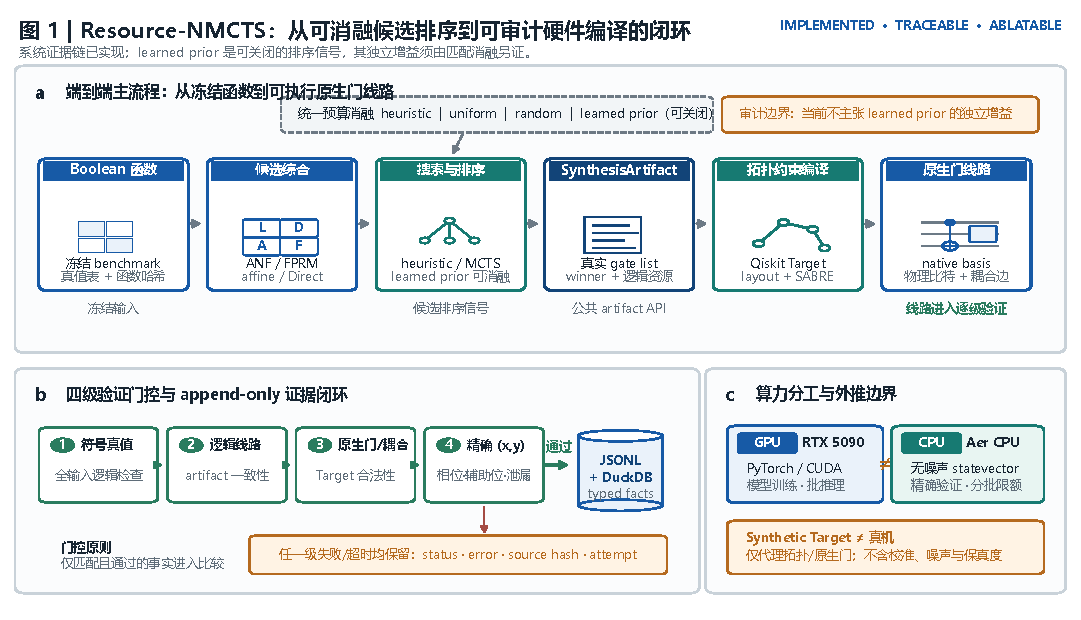
\includegraphics[width=\linewidth]{F2_system_architecture.pdf}
  \caption{\method{} 系统架构。Boolean 函数经表示与候选组合层生成逻辑线路，公共 artifact API 将同一门序列交给验证、synthetic Target 映射、图件生成和 DuckDB 归档。图中的 learned prior 是可选的监督训练动作评分器，而不是正确性判定器。}
  \label{fig:arch}
\end{figure}

\begin{enumerate}
  \item \textbf{表示与候选层：}真值表经快速 M\"obius 变换得到 square-free ANF；FPRM 极性和可逆仿射变换提供等价表示。候选包含透明直接基线、确定性因子搜索、MCTS 和结构化组合动作。
  \item \textbf{资源选择层：}每个正确候选报告逻辑 T、逻辑 CNOT、深度代理、门数和峰值辅助位；\method{} 在候选组合中按冻结 score 选择，并保留实际 \texttt{selected\_method}。
  \item \textbf{映射与验证层：}逻辑线路经显式 Qiskit Target、HLS、布局和 SABRE 路由形成原生门线路；验证器检查门集、耦合方向、全部输入态和相位一致性。
  \item \textbf{实验与审计层：}JSONL v3 逐行保存运行事实和资源遥测，DuckDB 保存规范化方法、target、attempt、mapping、verification 与 artifact provenance，冻结分析导出关联 analysis ID 和 SHA256。
\end{enumerate}

\FloatBarrier
\section{资源感知组合综合方法}
\label{sec:method}

\subsection{ANF/FPRM 状态与可验证动作}

输入函数表示为
\begin{equation}
  f(x)=\bigoplus_{m\in\mathcal{M}}\prod_{i\in m}x_i,
  \label{eq:anf}
\end{equation}
其中 $\mathcal{M}$ 是系数非零单项式的支撑集。FPRM 额外保存极性向量 $p\in\{0,1\}^n$，令 $z=x\xor p$，在保持函数语义不变的前提下寻找项数更少或更易分解的表示。输出逻辑线路仅使用 X、CNOT 和多控 Toffoli（MCT）抽象门。

搜索动作把当前项集合拆成 quotient 与 rest，递归构造 compute/reuse/uncompute 计划。公共单项式、FPRM 极性、线性奇偶因子和布尔环线性因子构成动作族。布尔环动作允许因子与 quotient 共享变量，并利用 $x_i^2=x_i$ 与 GF(2) 偶数项消去，例如
\begin{equation}
  (x_i\xor x_j)x_i m=x_i m\xor x_i x_jm.
  \label{eq:boolean-ring}
\end{equation}
这些动作可展开回 ANF，因此可在不依赖神经模型的条件下审计其代数语义。

\subsection{候选组合与 MCTS}

\method{} 是资源感知组合综合器，而不是单一神经网络算法。请求方法 \texttt{resource\_nmcts} 会运行适合当前规模的 Direct-ANF、FPRM/仿射候选、因子分解、cube 搜索和 MCTS 子方法；仅保留通过逻辑验证的候选，再以冻结资源 score 选择输出。组合结果必须同时记录请求方法和 \texttt{selected\_method}，从而区分“组合系统获益”和“某一学习模块获益”。

MCTS-Factor 使用启发式先验和有限 simulation budget，因而寻找的是低成本候选而非可证明全局最优解。Direct-ANF 始终提供透明参考；组合系统的 baseline-preserving 选择保证的是冻结加权 score 不劣于已成功的候选，而不是每个单项资源都同时占优。

\subsection{监督训练动作评分器}

正式 learned prior 为 \texttt{ActionNet}：24 维动作特征依次经过三个 96 单元隐藏层和一个标量输出层，即 $24\to96\to96\to96\to1$。模型使用 1,416 个按 truth-table SHA256 隔离的 Boolean functions 产生 1,623,060 条动作记录，并以 immediate-label regression 训练；checkpoint 为 \path{models/action_scorer_competition.pt}，SHA256 为 \texttt{6ba157fb9b5504d815d250ce55bb7d6509bce05ead24547e07dc6644ba8b3617}。训练使用 RTX 5090 Laptop GPU，小批搜索推理默认使用 CPU。

候选先验按
\begin{equation}
  p(a\mid s)=h(a\mid s)+1.0\,s_{\mathrm{NN}}(a\mid s)
  \label{eq:prior}
\end{equation}
组合，其中 $h$ 是确定性资源启发式，$s_{\mathrm{NN}}$ 是标准化后的模型输出。heuristic-only 保留 $h$；uniform prior 替换而不是删除启发式路径；random prior 使用固定 seed 的哈希分数。四组消融保持候选宽度、simulation budget 和综合 seed 一致。

\subsection{资源模型与主指标}

资源安全主 runner 的候选排序 score 为
\begin{equation}
  \mathrm{score}=1.0T+0.04\,\mathrm{CNOT}+0.015\,\mathrm{depth}
  +0.01\,\mathrm{gates}+2.0\,\mathrm{ancilla}.
  \label{eq:score}
\end{equation}
该式只用于逻辑候选排序，不代表设备运行时间或物理错误率。库默认值及 learned-prior 训练标签使用 $0.05$ 的 CNOT 权重和 $0.02$ 的 depth 权重；训练配置与正式评估配置均写入 manifest。为避免 score 定义影响主结论，正式预注册指标分别为逻辑 T、逻辑 CNOT、native-2Q 和 mapped depth，score 仅作次要分析。

\subsection{验证门槛}

综合 artifact 首先通过 \texttt{verify\_oracle()} 对全部 $2^n$ 个输入进行位并行精确检查，验证输出真值表、输入保持和辅助位归零。代码库另提供 factor-plan ANF 展开和 emitted-circuit GF(2) 符号检查，用于回归测试与实例审计；未接入某一正式 runner 时，不把它们写成该批次的强制门槛。

映射后验证按 initial/final layout 枚举全部 $2^{n+1}$ 个 $(x,y)$ 基态，检查数据位、Oracle 输出、辅助位、泄漏和输入相关相位。只有逻辑验证、原生门/耦合检查和映射后精确验证同时通过的行，才进入质量统计。

\section{系统实现与数据治理}

公共入口 \texttt{synthesize\_artifact(method, bf, config, seed, model\_path)} 返回标量资源、真实逻辑门序列和 \texttt{selected\_method}；旧入口 \texttt{synthesize()} 与其共享同一执行路径。\path{src/hardware_map.py} 负责 Target 构造、HLS、布局、路由、指标与映射验证，避免图件、仿真和统计各自重建线路。

正式基线统一通过同一调度接口运行：Direct-ANF、Greedy-Factor、MCTS-Factor、SSHR-H、SSHR-Beam 与 \method{}。其中 SSHR-H 是对论文启发式流程的本地复现；SSHR-Beam 是在相同 parallelotope 表示上实现的固定宽度 beam-search 扩展，并非论文中依赖 Gurobi 的 ILP 版本 SSHR-I。冻结 primary20 未运行 SSHR-I，因而正文只比较本地 SSHR-H/Beam，不声称超过论文完整方法。ESOP/MILP、cube 及外部 ABC/mockturtle/CirKit/RevKit/Caterpillar 对接脚本保留为扩展能力；若没有同任务、同辅助位和同超时条件的重跑结果，则只用于能力说明或相关工作定位，不进入主胜负表。

实验 runner 采用 append-only JSONL v3。每个 stage 保存函数哈希、方法、seed、配置、模型哈希、target、线路哈希、耗时、worker 进程树 RSS 与系统内存峰值。DuckDB schema 将实验、方法规格、综合 attempt、映射、验证和 artifact 分表保存；恢复运行按 semantic cell 去重，质量视图取最早的验证成功 attempt，原始超时与失败仍保留在 JSONL 和 recovery manifest 中。

\section{硬件兼容性与本地仿真}
\label{sec:hw}

\subsection{机器、软件与加速边界}

\begin{table}[H]
  \centering
  \footnotesize
  \caption{本地机器与冻结软件栈。设备名称不等同于所有阶段都由 GPU 加速。}
  \label{tab:environment}
  \begin{tabularx}{\linewidth}{>{\bfseries}p{0.25\linewidth}Y}
    \toprule
    项目 & 实测配置与使用边界 \\
    \midrule
    CPU/内存 & 24 个逻辑处理器，约 63.4 GB 物理内存 \\
    GPU & NVIDIA GeForce RTX 5090 Laptop GPU，24,463 MiB；用于模型训练和适合的批评分 \\
    Python/PyTorch & Python 3.11.15；PyTorch 2.9.1+cu128；CUDA runtime 12.8 \\
    Qiskit & Qiskit 2.5.0；Qiskit Aer 0.17.2 \\
    Aer 设备 & 当前 \texttt{available\_devices} 只有 CPU；状态仿真未使用 RTX 5090 \\
    数据库 & DuckDB 1.5.4 \\
    \bottomrule
  \end{tabularx}
\end{table}

状态向量验证随物理比特指数增长，因此冻结协议仅对 $n\leq8$ 执行全部 $(x,y)$ 输入态；超过该边界时，当前实现拒绝把抽样结果标为 exact。正式恢复批次使用 batch size 16、Aer threads 16、parallel experiments 16、worker 每 8 个 stage 回收和 70\% 系统内存软上限。AES Direct 单例的 runner 工程测试中，有界实验并行把精确验证从 187.3 s 降至 103.4 s（1.81 倍），系统内存约为 27\%；该数字只描述本地运行器加速，不是量子线路质量提升。

\subsection{synthetic Target 与映射语义}

代码支持全连接/线形 CX、二维 CZ grid 和 ECR heavy-hex synthetic Target。资源安全主分析实际冻结为 \texttt{cx\_full\_12}；四比特线形实例用于展示稀疏路由，grid/heavy-hex 在进入统一实验前只称“实现支持”。这些 Target 没有门时长、读出误差、串扰、漂移或校准时间戳，因此只能报告原生门数、native-2Q、深度、routing delta 和无噪声等价。

\begin{table}[H]
  \centering
  \footnotesize
  \caption{synthetic Target 的实现与证据状态。正式主分析与实例图不可跨行合并解释。}
  \label{tab:targets}
  \begin{tabularx}{\linewidth}{>{\bfseries}p{0.25\linewidth}p{0.22\linewidth}Y}
    \toprule
    Target & 当前状态 & 可支持的表述 \\
    \midrule
    \texttt{cx\_full\_12} & 冻结主分析 & 无校准全连接 CX 参考；可作统一映射比较 \\
    \texttt{cx\_line\_4\_bidir} & \texttt{maj3} 实例 & 稀疏路由与映射后 exact 验证，不代表总体结果 \\
    CZ grid & 代码支持 & 可构造、编译与检查；尚非冻结主分析 \\
    ECR heavy-hex & 代码支持 & 可构造、编译与检查；尚非冻结主分析 \\
    \bottomrule
  \end{tabularx}
\end{table}

\begin{figure}[p]
  \centering
  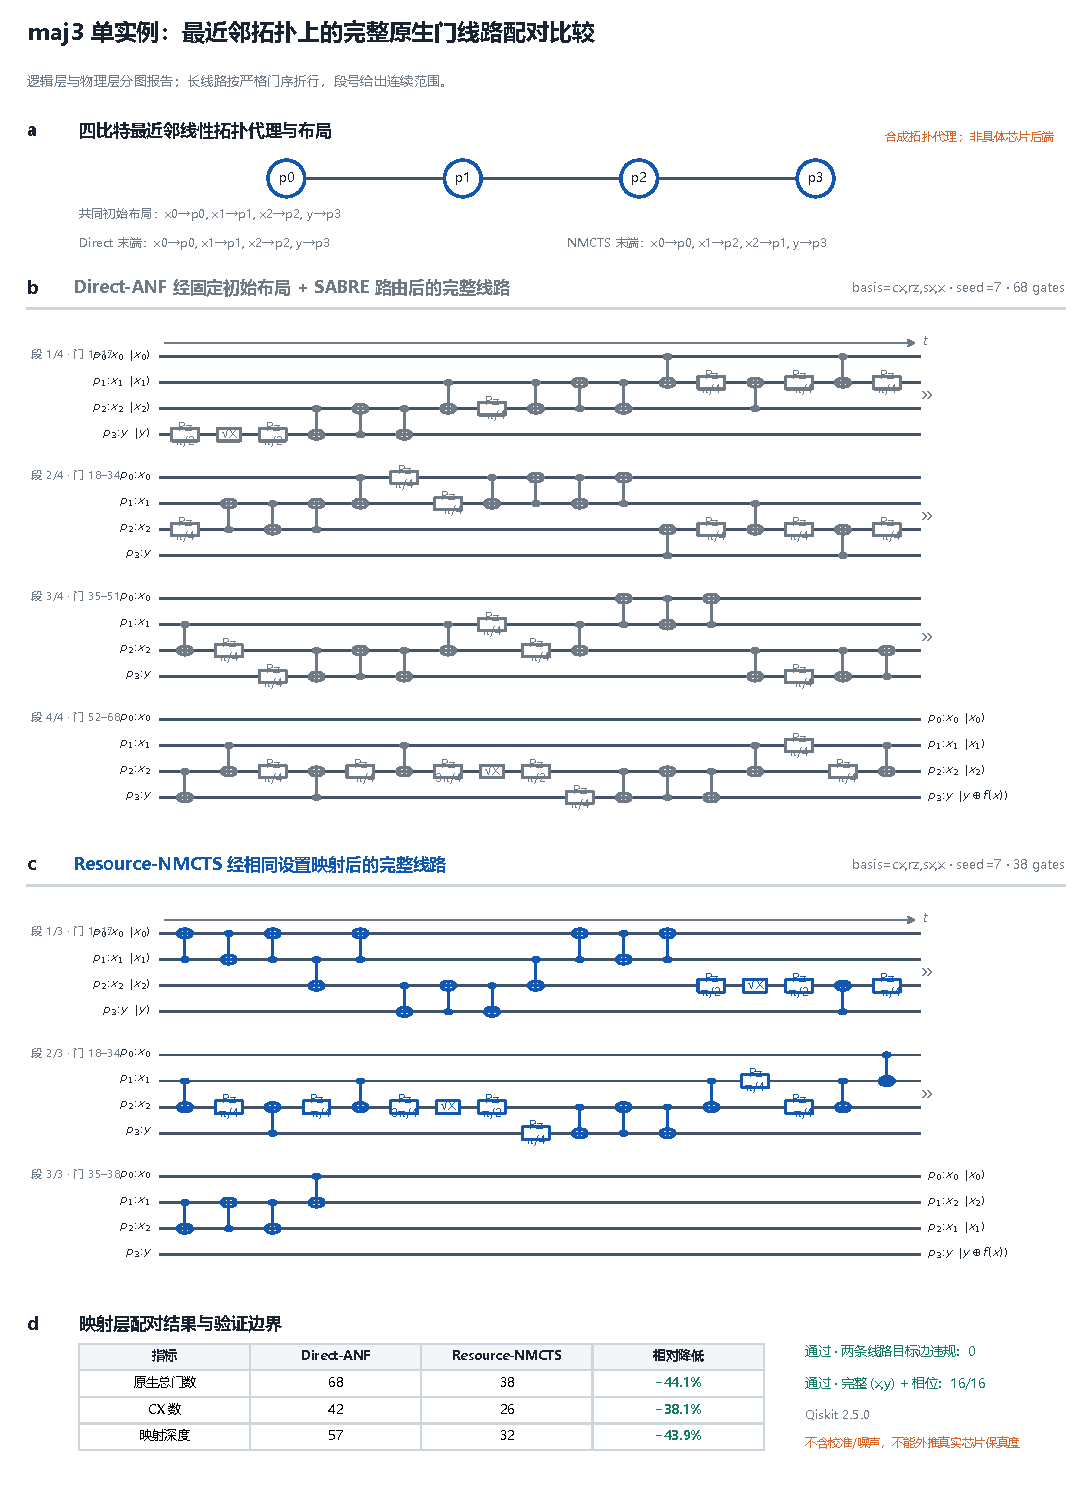
\includegraphics[width=0.94\linewidth,height=0.80\textheight,keepaspectratio]{F1_standard_hardware_mapping.pdf}
  \caption{程序生成的 \texttt{maj3} 硬件映射实例。\method{} 请求最终选择 \texttt{affine\_greedy}；Target 为无校准 \texttt{cx\_line\_4\_bidir}，映射线路通过原生门、耦合边与全部 16 个 $(x,y)$ 输入态的精确验证。图中改善是单实例组合选择结果，不能归因于 learned prior，也不能解释为真实芯片保真度提升。}
  \label{fig:mapping}
\end{figure}

高控制 MCX 的 HLS 曾暴露一项关键兼容性问题：若笼统声明所有 qubit 初始为零，Qiskit 可能把任意数据线当作 clean ancilla，产生门集合法但 Oracle 语义错误的线路。现实现只把显式新增的 \texttt{AncillaRegister} 交给 clean-ancilla 分解，并在后续 pass manager 中固定 \texttt{qubits\_initially\_zero=False}；回归测试对任意输入态重新验证。这一案例说明硬件兼容性必须包含语义验证，而不能止于 transpile 成功。

图~\ref{fig:mapping} 展示同一 \texttt{maj3} 实例从逻辑线路到四比特双向线形 CX Target 的编译。该图是 synthetic line pilot，不代表校准真机或正式 \texttt{cx\_full\_12} 总体结果。

\FloatBarrier
\section{实验结果与比较协议}
\label{sec:results}

\subsection{可复现实例}

图~\ref{fig:oracle-example} 对比同一 \texttt{maj3} Boolean function 的 Direct-ANF 与 \method{} 逻辑线路。所有线路来自公共 artifact API，而非为绘图手工重建。表~\ref{tab:worked-example} 汇总同一实例在逻辑层和 line synthetic Target 上的资源。

\begin{table}[H]
  \centering
  \footnotesize
  \caption{\texttt{maj3} 单实例资源；映射列对应 \texttt{cx\_line\_4\_bidir}，不是冻结主分析 Target。}
  \label{tab:worked-example}
  \begin{tabular}{lrrrrr}
    \toprule
    方法 & T & CNOT & 原生 2Q & 映射深度 & exact states \\
    \midrule
    Direct-ANF & 12 & 18 & 42 & 57 & 16/16 \\
    \shortstack[l]{\method{}\\\texttt{affine\_greedy}} & 4 & 11 & 26 & 32 & 16/16 \\
    \bottomrule
  \end{tabular}
\end{table}

\begin{figure}[p]
  \centering
  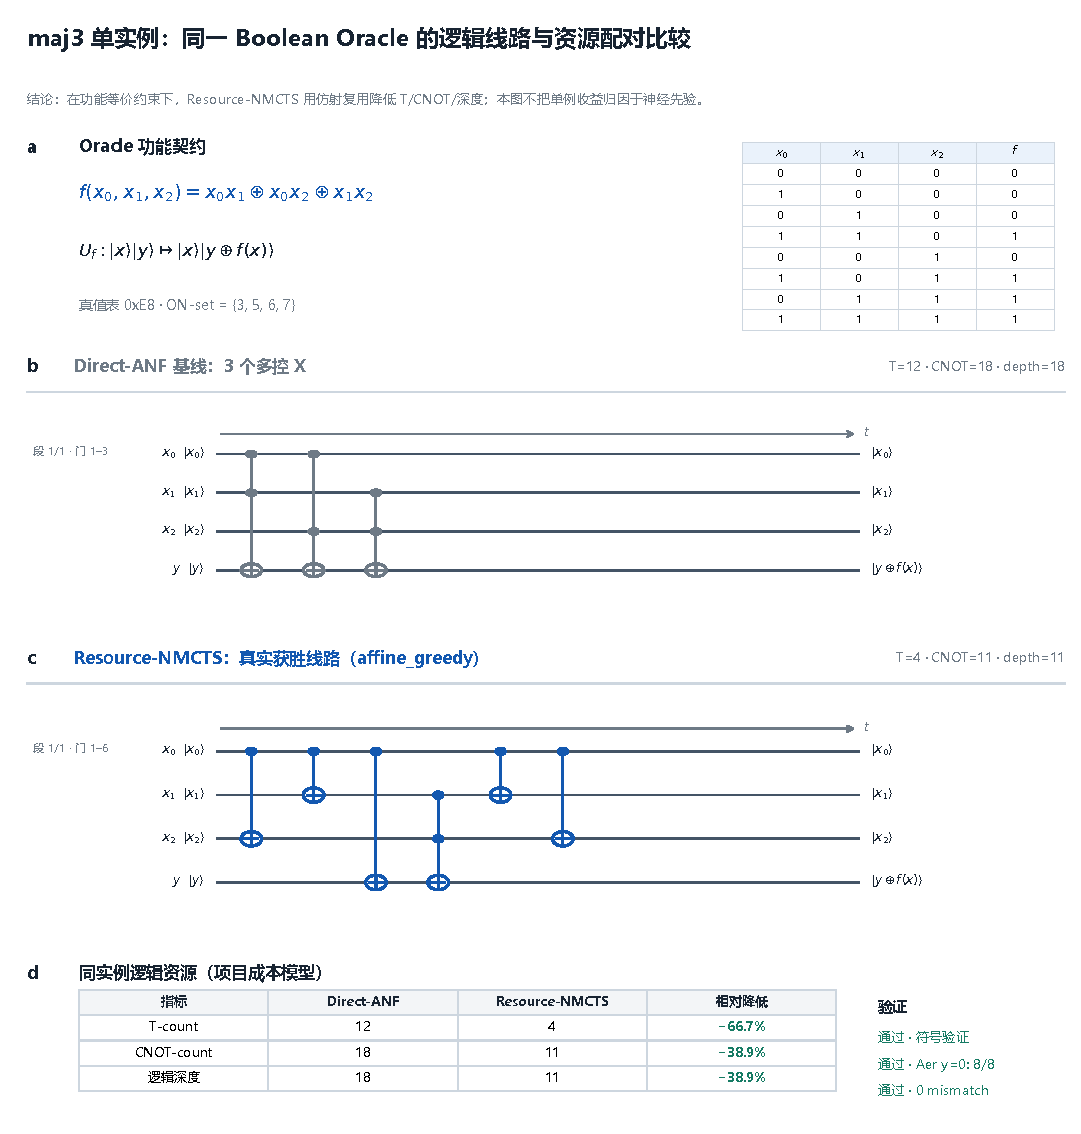
\includegraphics[width=0.92\linewidth,height=0.70\textheight,keepaspectratio]{F0_standard_oracle_comparison.pdf}
  \caption{\texttt{maj3} 的程序生成逻辑线路。Direct-ANF 与 \method{} 使用相同函数和综合 seed 7；\method{} 的 \texttt{selected\_method} 为 \texttt{affine\_greedy}。该图证明实例、线路和指标可由统一 API 复现，不构成 learned prior 的独立消融证据。}
  \label{fig:oracle-example}
\end{figure}

\subsection{冻结主分析与 coverage}

总体比较遵循冻结实验协议（\path{EXPERIMENT_PROTOCOL.md}）。表~\ref{tab:coverage-contract} 给出不会随恢复顺序改变的 coverage 分母。失败、超时、中断和缺 seed 保留在 coverage/failure 输出中；质量统计仅使用 candidate 与 baseline 都满足三个指定 seed 的函数。

\begin{table}[H]
  \centering
  \small
  \caption{资源安全主分析的冻结 coverage 结构。}
  \label{tab:coverage-contract}
  \begin{tabularx}{\linewidth}{>{\bfseries}p{0.26\linewidth}Y}
    \toprule
    维度 & 冻结设置 \\
    \midrule
    Boolean functions & 20：8 structured、6 random-truth、4 random-ANF、2 AES；$n=3\ldots8$ \\
    方法 & Direct-ANF、Greedy-Factor、MCTS-Factor、SSHR-H、SSHR-Beam、\method{} \\
    综合 seeds & $\{7,17,29\}$；同一函数三个 seed 全部成功才进入正式推断 \\
    计划逻辑单元 & $20\times6\times3=360$ 个 semantic cells \\
    映射配置 & \texttt{cx\_full\_12}，transpiler seed 3，optimization level 1，SABRE，HLS ancilla budget 0 \\
    正确性 & 逻辑穷举、原生门/耦合零违规、映射后全部 $(x,y)$ 精确验证 \\
    统计单位 & Boolean function；seed 先在函数内配对并取中位差 \\
    多重比较 & logical primary 与 mapping primary 分族 Holm；另报 global Holm 敏感性 \\
    \bottomrule
  \end{tabularx}
\end{table}

冻结分析标识为 \texttt{\FinalAnalysisID}。clean DuckDB 的 SHA256、五组只读统计输入、coverage audit 和输出哈希记录在 \path{submission_competition/final_analysis_manifest.json}；统计脚本确认分析前后数据库字节哈希一致。图~\ref{fig:coverage-resource} 显示完整分母：\FinalPlannedCells{} 个计划单元中 \FinalVerifiedCells{} 个通过（\FinalCoveragePct\%）。SSHR-Beam 在两个 AES 分量上的早期 $n=8$ 综合超时已通过 quad 向量化补全，\FinalMissingCells{} 个缺口；没有 truth-table mismatch、非法耦合、unsupported instruction 或内存保护触发。

\begin{figure}[p]
  \centering
  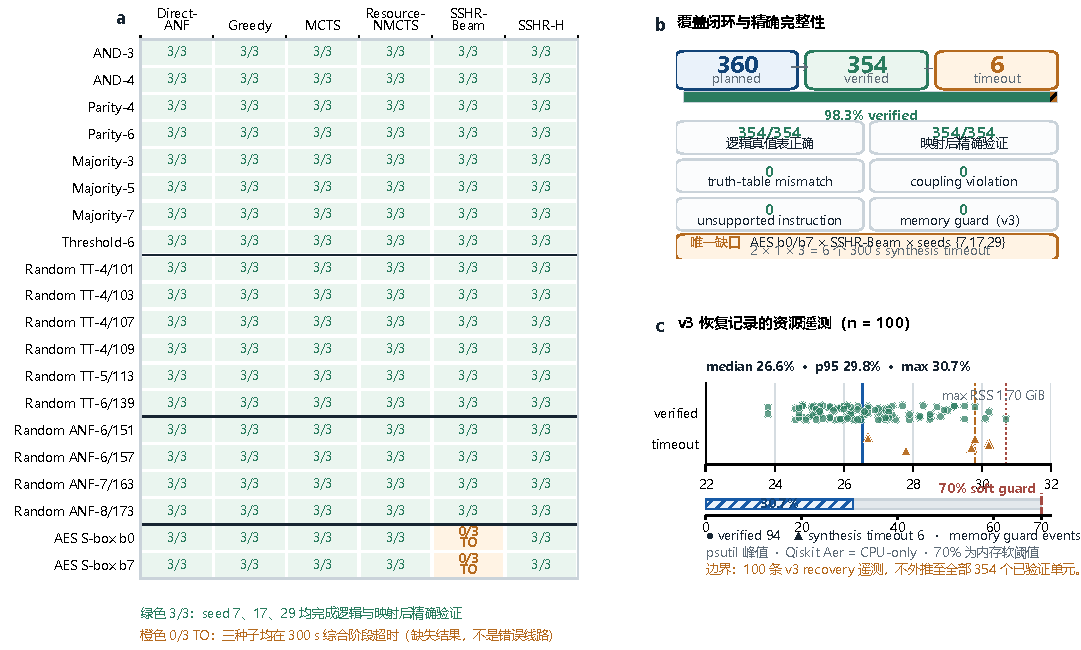
\includegraphics[width=\linewidth]{F5_coverage_correctness_resource.pdf}
  \caption{冻结 coverage、正确性与资源安全审计。\textbf{a} 20 个 Boolean 函数、6 个方法和 3 个 seed 的矩阵；绿色 $3/3$ 表示逻辑与映射后精确验证均完成（360/360 全部完成，无超时缺口）。\textbf{b} 计划、成功与失败分母及正确性检查。\textbf{c} 针对恢复记录的 psutil 遥测：系统内存峰值软阈值为 70\%；Qiskit Aer 为 CPU-only。Source data are provided in the figure source CSV/JSON.}
  \label{fig:coverage-resource}
\end{figure}

表~\ref{tab:primary-results} 和图~\ref{fig:primary-results} 报告全部五个强基线，而不是只展示胜项。主效应量为函数内三个严格配对 seed 的中位差，再在独立函数上取中位相对改善；95\% 区间由 20,000 次固定 seed bootstrap 得到。严格“显著优于”要求方向有利、分族 Holm 拒绝、raw median $\Delta$ 区间上界 $<0$，且中位相对改善区间下界 $>0$；触及 0 也按中性处理。

\begin{table}[tbp]
  \centering
  \scriptsize
  \caption{\method{} 相对五个基线的冻结主指标。单元为中位相对改善\% [95\% bootstrap CI]，正值有利于 \method{}；粗体满足严格门槛。$\dagger$ 表示分族 Holm 已拒绝，但至少一个中位效应区间触及或跨越 0，故不称严格显著。}
  \label{tab:primary-results}
  \resizebox{\linewidth}{!}{%
  \begin{tabular}{lccccc}
    \toprule
    基线 & $n$ & 逻辑 T & 逻辑 CNOT & native-2Q & mapped depth \\
    \midrule
    Direct-ANF & 20 & \textbf{51.5 [39.1, 61.1]} & \textbf{16.6 [4.9, 23.7]} & \textbf{42.0 [7.5, 67.5]} & \textbf{45.2 [6.1, 71.7]} \\
    Greedy-Factor & 20 & \textbf{23.6 [17.3, 34.4]} & $18.1 [0.0, 23.0]^{\dagger}$ & $16.1 [0.0, 22.8]^{\dagger}$ & $16.9 [0.0, 25.1]^{\dagger}$ \\
    MCTS-Factor & 20 & \textbf{23.6 [15.5, 34.4]} & $19.6 [0.0, 22.8]^{\dagger}$ & $12.8 [0.0, 22.8]^{\dagger}$ & $10.3 [0.0, 25.1]^{\dagger}$ \\
    SSHR-H & 20 & $10.0 [-5.3, 29.2]$ & $-28.0 [-54.5, 0.0]$ & \textbf{30.6 [3.0, 40.2]} & $38.3 [-0.9, 47.7]^{\dagger}$ \\
    SSHR-Beam & 20 & \textbf{40.9 [21.2, 50.0]} & $-7.1 [-39.8, 12.1]$ & \textbf{45.3 [34.1, 50.5]} & \textbf{51.8 [40.6, 55.7]} \\
    \bottomrule
  \end{tabular}}
\end{table}

相对 Direct-ANF，四个预注册主指标全部严格支持改善，胜/平/负依次为 T 的 $17/3/0$ 和其余三项的 $14/3/3$，最大分族 Holm $p_{\mathrm H}=0.00184$。相对 Greedy-Factor 和 MCTS-Factor，逻辑 T 的严格改善均为 23.6\%；其他三项的 Holm 检验支持方向性差异，但中位区间触 0。相对 SSHR-H，只有 native-2Q 的 30.6\% 改善满足严格门槛；逻辑 T/CNOT 不显著，mapped depth 的区间跨 0。SSHR-Beam 的两个 AES 函数在补全 quad 向量化后已三 seed 全部完成，比较覆盖全部 $n=20$；在该完整集合上逻辑 T、native-2Q 和 mapped depth 严格改善，逻辑 CNOT 为负中位改善且不显著。由此，本项目可以在上述限定指标与基线上使用“显著优于”，但不能声称全基线、全指标支配。

\begin{figure}[p]
  \centering
  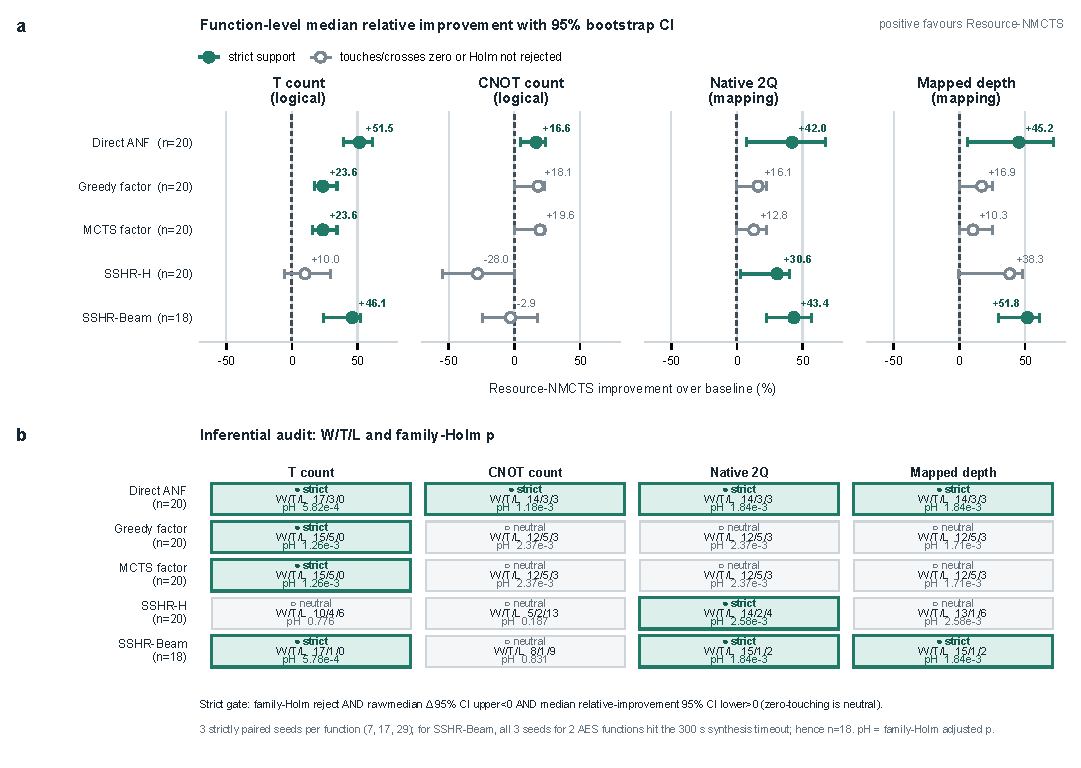
\includegraphics[width=\linewidth]{F4_frozen_primary_results.pdf}
  \caption{冻结主结果与推断审计。\textbf{a} \method{} 相对五个基线的函数级中位相对改善及 95\% bootstrap CI，正值有利；实心绿色仅标记同时通过双区间与分族 Holm 门槛的比较。\textbf{b} 每格给出独立函数数、胜/平/负和分族 Holm 校正 $p_{\mathrm H}$。每个函数先严格配对 seed 7/17/29；SSHR-Beam 比较覆盖全部 $n=20$（两个 AES 分量经 quad 向量化补全后三 seed 均完成）。Source data are provided in the figure source CSV/JSON.}
  \label{fig:primary-results}
\end{figure}

\subsection{AI 消融与归因}

learned prior 的正式因果问题是：在相同动作集合、候选宽度、simulation budget 和 seed 下，它是否优于 heuristic-only、uniform prior 与 random prior。代码路径在 $n\geq6$ 时跳过神经评分，因此这些函数上的结果不能归因于 learned prior。

完整 primary20 中共有 60 个成功 \method{} 单元：54 个明确选择 \texttt{direct\_anf}、\texttt{fprm\_greedy}、\texttt{fprm\_linear\_pair} 或 \texttt{affine\_greedy} 等确定性分支；其余 6 个选择 \texttt{affine\_nmcts}，也只能称“可能受 learned prior 影响”，不能据方法名断言因果贡献。独立 clean pilot 含 8 个匹配单元：learned 与 heuristic、uniform、rollout 三个对照均为 $0/8/0$；相对 random 为 $2/6/0$，逻辑 T/CNOT 的双侧 Wilcoxon 均为 $p=0.5$。hard3 反例中 immediate 与 rollout 的收益混合，映射深度还可整体退化，运行时间中位数分别达到 heuristic 的 3.8 倍与 12.0 倍。图~\ref{fig:ai-attribution} 因而把训练事实、同预算 pilot、反例和组合归因边界放在同一证据链中。主结果使用的 method identity 为 \texttt{model-configured}，不是 \texttt{learned}；本文不把组合收益归因于神经网络，负结果也不隐藏。

\begin{figure}[H]
  \centering
  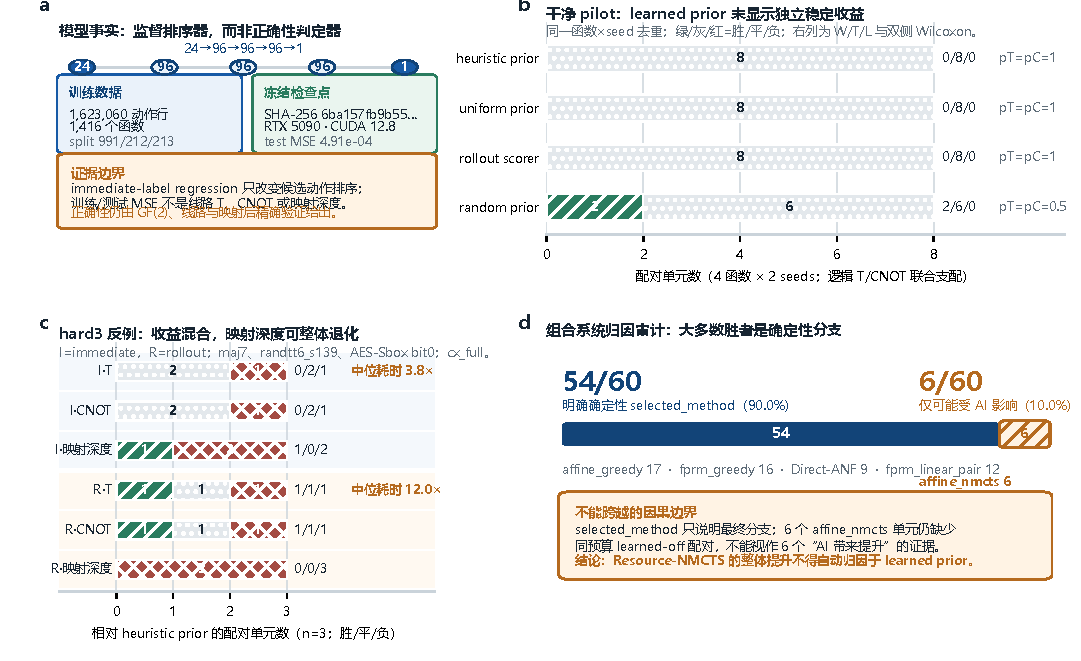
\includegraphics[width=\linewidth]{F3_ai_ablation_attribution.pdf}
  \caption{学习模块的消融与归因边界。\textbf{a} 24--96--96--96--1 监督评分器只改变候选排序，训练/test MSE 不是线路资源或正确性证据。\textbf{b} clean pilot 在同函数、同 seed、同预算下比较 learned 与 heuristic、uniform、rollout、random prior；条形为胜/平/负，$n=8$。\textbf{c} 三个 hard cases 的逐指标反例与相对运行时间。\textbf{d} 60 个冻结 \method{} 单元中 54 个选择明确确定性分支，6 个 \texttt{affine\_nmcts} 仍缺 learned-off 配对。该图不支持 learned prior 的稳定独立收益。Source data are provided in the figure source CSV/JSON.}
  \label{fig:ai-attribution}
\end{figure}

\FloatBarrier
\section{相关工作与文献综述}
\label{sec:related}

相关研究可按编译抽象层分为三类：从 Boolean 函数生成可逆 Oracle 的逻辑综合、以
MCTS 或学习模型控制离散线路搜索、以及在给定逻辑线路后执行的布局与路由。三类工作
的输入对象、允许门集和评价指标不同。本节因而先比较机制与适用范围，再说明可执行的
公平对比条件，不把跨抽象层的作者报告数字直接并列。

\subsection{Boolean Oracle 的逻辑表示与综合}

早期可逆逻辑综合主要从规范逻辑表示构造 Toffoli 级联。Gupta 等利用正极性
Reed--Muller 展开搜索多输出间的公共因子\cite{gupta2006pprm}；ESOP-to-Toffoli
方法把积项直接映射为可逆门级联\cite{fazel2007esop}；BDD 路线则以图分解换取对较大
函数的处理能力\cite{wille2009bdd}。面向 Oracle 嵌入的自动化研究还区分最少 qubit 与
保留函数 domain 的实现\cite{henderson2023minimal}。这些方法共同说明，逻辑表示、寄存器
语义、变量序和因子复用
会直接改变 MCT 数量及其控制数分布。对本项目而言，Direct-ANF/ESOP、PPRM 因子搜索
和 BDD 因而分别构成透明直接基线、代数结构基线与规模扩展参照；但一般可逆置换与式
~\eqref{eq:oracle} 的单输出 bit-flip Oracle 并非完全相同，比较时还必须统一负控制、
辅助比特和 MCT 分解规则。

面向容错资源的现代 Oracle 综合进一步显式区分 XOR 与非线性运算。乘法复杂度工作把
XOR--AND 网络中的 AND 数与 T-count、辅助比特开销联系起来，并研究空间--T
交换\cite{meuli2019multiplicative}；ROS 以资源感知 LUT mapping 和 SAT garbage
management 综合受限资源下的 Oracle\cite{meuli2020ros}；XAG 编译则在统一逻辑网络
中探索 qubit、T-count 与 T-depth 的权衡\cite{meuli2022xag}。近期研究开始把容错后端
代价前置到 XAG 优化\cite{yu2025backend}，SSHR 则针对 $n\leq8$ 的 Boolean 函数，
利用超立方体中的 parallelotope 结构减少 MCT/CNOT 资源，并给出启发式和 ILP
变体\cite{zheng2025sshr}。本文的 SSHR-H 是启发式复现，SSHR-Beam 是本地 beam-search
扩展而不是论文 SSHR-I；未运行的 ILP 版本不进入胜负结论。其中 ROS、XAG 与 SSHR 是本项目最接近的任务级参照；本项目的
区别在于以可展开回 ANF/FPRM 的 factor plan 为动作空间，由资源约束 MCTS 选择
compute/reuse/uncompute 计划。该区别只说明搜索空间和控制机制不同；只有在同一真值
表、Oracle 语义、辅助比特规则、门分解、超时与随机种子下重跑，才可形成定量胜负。

\subsection{MCTS 与学习引导的线路搜索}

MCTS 和学习模型已被用于多种线路设计与综合任务。Nested MCTS
\allowbreak\cite{wang2023nestedmcts} 可自动设计面向量子化学、图优化等任务的参数化线路；
QSeed\allowbreak\cite{weiden2023qseed} 用学习模型为 bottom-up unitary synthesis 提供初始候选；
Gumbel AlphaZero\allowbreak\cite{rietsch2024rlsynthesis} 已用于离散 Clifford+T 门集上的精确
unitary synthesis。

与 Boolean 表示更接近的 ShortCircuit\allowbreak\cite{tsaras2024shortcircuit} 从真值表生成经典
AIG，但其当前可核验版本为预印本，且不承担量子可逆化、辅助比特清理或 T/CNOT 成本。
扩散模型\allowbreak\cite{fuerrutter2024diffusion} 能够条件生成和编辑量子线路；
AlphaTensor-Quantum\allowbreak\cite{ruiz2025alphatensor} 从已有 CNOT+T 线路的非 Clifford 部分
出发优化 T-count；RL-ZX\allowbreak\cite{riu2025rlzx} 则学习选择保持等价的 ZX 图重写；近期
强化学习还被用于在连通性和门集约束下发现容错逻辑态制备线路\cite{zen2025rlft}。这些工作
分别属于生成式综合或后综合优化，不能直接替代从 Boolean 函数到精确 bit-flip Oracle
的前端。

因此，本项目的 AI 定位不是“首次把 MCTS/RL 用于线路综合”，而是把学习先验约束在
Boolean Oracle 的可验证代数动作上。相应实验必须在同一候选集合、simulation budget
和 seed 下比较 heuristic、uniform、random-prior 与 learned-prior，并把完整组合系统
的收益与神经先验的增量分开报告。一般 unitary、经典 AIG 或已有线路重写上的速度与门数
结果只能支持方法动机，不能作为本项目优于同任务 Oracle 综合器的证据。

\subsection{拓扑映射、路由与硬件感知编译}

布局与路由以已经生成的逻辑线路为输入，解决的是另一层优化问题。SABRE 通过启发式
双向搜索联合改进初始布局和 SWAP 路由\cite{li2019sabre}；路由问题的形式化研究进一步
明确了架构图、允许原语和调度规则对成本的影响\cite{cowtan2019routing}；整数规划方法
可在小规模上联合求解分配与路由，并提供最优解或 optimality
gap\cite{nannicini2022ilp}。在仅有 coupling map 之外，noise-adaptive mapping 使用设备
校准信息选择更可靠的实现\cite{murali2019noiseadaptive}，学习排序方法则利用真实硬件
数据在多个逻辑等价布局中选择候选\cite{hartnett2024learningtorank}。HOPPS 进一步把任意拓扑
约束前置到 $\{\mathrm{CNOT},R_z\}$ phase-polynomial block 的 SAT/分块综合中
\cite{li2025hopps}，但其门集与本文 bit-flip 前端不同，且当前仅作为预印本边界。

这些工作给出了硬件层的必要对照，也限定了本文可使用的表述：固定同一 basis-decomposed
逻辑线路后，才能比较 native-2Q、二比特门深度、routing delta 与编译时间；只有具备带
时间戳的校准或真实执行数据时，才能讨论噪声感知排序和硬件性能。本项目据此把逻辑综合、
topology-aware mapping 与 calibration-aware compilation 分层记录。synthetic line/grid/
heavy-hex 耦合图上的本地结果属于拓扑压力测试，不能被表述为真实设备保真度提升，也不能
用来替代容错后端中的 T-count、logical time step 或 QEC 资源比较。

\section{贡献、应用与限制}

\subsection{可审计的工程与方法贡献}

\begin{enumerate}
  \item 将 bit-flip Boolean Oracle 的 ANF/FPRM 等价表示、因子动作和 compute/uncompute 计划统一到可展开、可验证的离散搜索接口中。
  \item 实现资源感知候选组合与公开 artifact API，保留真实门序列和 \texttt{selected\_method}，使综合、映射、仿真、图件和数据库共享同一事实源。
  \item 将监督训练动作评分器限制为可替换的排序模块，并设计 heuristic、uniform、random 与 learned 的同预算消融；当前负结果被作为方法边界而非隐藏项报告。
  \item 实现显式 Target、HLS ancilla、SABRE 路由、原生门/耦合检查与映射后全输入相位验证，修复了 MCX clean-ancilla 语义风险。
  \item 建立 JSONL v3、DuckDB、恢复去重、函数级统计、资源遥测和 artifact hash 组成的竞赛级审计链。
\end{enumerate}

\subsection{可支持的应用范围}

当前实现适用于可由真值表或 ANF 给出的 bit-flip Boolean predicates。AES S-box 单输出分量被纳入冻结 benchmark，用于检验密码学相关非线性函数，而不是宣称已经完成整个 AES 密钥搜索 Oracle 或 QEC 资源估算。Grover 型约束搜索可以复用同一 bit-flip 接口，但规模受真值表和精确验证的指数成本限制。该系统还可作为学习引导组合搜索、编译器正确性和拓扑映射的教学/研究平台。

接入真实量子云平台需要新增 provider/backend 身份、带时间戳的 Target 与 properties、noise-model hash、shot 协议和设备日志。在这些证据落盘之前，天衍等真机只作为可执行路线，而不是本文已经完成的实验。

\subsection{已知瓶颈}

\begin{itemize}
  \item \textbf{SSHR-Beam 的 n=8 性能边界：}SSHR-Beam 在 $n\geq8$ 上曾因逐元素 Python 掩码循环而在 AES 分量上综合超时；本作品已为其增加 4-lane uint64 向量化路径补全至 360/360，但该基线在大函数上仍可能受束宽与候选枚举开销限制。
  \item \textbf{learned prior 增益有限：}先导消融尚未观察到稳定独立收益；组合系统的优势可能主要来自表示变换和确定性候选。
  \item \textbf{硬件模型有限：}当前仅有无校准 synthetic Target 和无噪声 CPU Aer，不能推断真实保真度、时长或 QEC 总成本。
  \item \textbf{精确验证指数扩展：}正式全 $(x,y)$ 验证限定在 $n\leq8$；更大规模需把符号证明、抽样验证和适用边界分别报告。
  \item \textbf{辅助位与版本敏感：}高控制 MCX 的分解依赖显式辅助位预算；Qiskit、HLS 与 SABRE 的版本和 seed 会改变映射结果。
  \item \textbf{门集范围：}核心引擎没有独立 Rz 旋转或一般相位 Oracle 综合后端。
\end{itemize}

\section{结论}

本文完成了从 Boolean 函数、资源感知组合综合、synthetic Target 映射、本地精确验证到 DuckDB 审计的闭环。冻结分析 \texttt{\FinalAnalysisID} 在 360/360 个计划单元上形成可追溯证据；相对 Direct-ANF，逻辑 T/CNOT、native-2Q 与 mapped depth 四个主指标分别严格改善 51.5\%、16.6\%、42.0\% 和 45.2\%。更强基线揭示了真实边界：Greedy/MCTS 只有逻辑 T 严格改善，SSHR-H 只有 native-2Q，SSHR-Beam 的完整 20 函数上有三项严格改善而 CNOT 不占优。完整组合中 54/60 个输出来自确定性分支，clean learned-prior pilot 未显示稳定独立收益。因此可支持的结论是“在冻结匹配协议的若干主指标上显著优于对应基线”，而不是全指标支配、神经网络单独增益或真实硬件保真度提升。

\appendix
\section{运行与复现说明}
\label{app:repro}

\subsection{环境原则}

主环境为 conda 环境 \texttt{mcts-qoracle}。关键版本、GPU/Aer 能力、Python 包、代码与模型 SHA256 由 \path{submission_competition/environment_manifest.json} 和 \path{submission_competition/environment_packages.txt} 保存。发布文档不绑定开发机用户名或绝对解释器路径。

\subsection{冒烟测试}

在 PowerShell 中进入项目的 \path{resource_nmcts} 目录后执行：

\begin{lstlisting}
$env:KMP_DUPLICATE_LIB_OK = "TRUE"
conda run -n mcts-qoracle python tests/tests_smoke.py
\end{lstlisting}

\subsection{资源安全硬件验证示例}

下列命令展示冻结 runner 的关键资源参数；函数、方法与输出文件应由实验 manifest 指定。

\begin{lstlisting}[basicstyle=\ttfamily\scriptsize]
$env:KMP_DUPLICATE_LIB_OK = "TRUE"
conda run -n mcts-qoracle python scripts/run_hardware_validation.py `
  --suite final --functions maj3 `
  --methods direct_anf,resource_nmcts --seeds 7 `
  --targets cx_full --cx-qubits 12 `
  --transpile-seeds 3 --optimization-level 1 `
  --hls-ancilla-budget 0 --timeout 300 `
  --verification-batch-size 16 --aer-max-parallel-threads 16 `
  --aer-max-parallel-experiments 16 --worker-max-tasks 8 `
  --max-system-memory-percent 70 `
  --model-path models/action_scorer_competition.pt `
  --output-jsonl results/reproduction_smoke.jsonl
\end{lstlisting}

\subsection{文档编译}

在 \path{submission_competition} 目录执行完整参考文献链：

\begin{lstlisting}
xelatex -interaction=nonstopmode main.tex
bibtex main
xelatex -interaction=nonstopmode main.tex
xelatex -interaction=nonstopmode main.tex
\end{lstlisting}

\begingroup
\footnotesize
\setlength{\bibsep}{1.5pt plus 0.2ex}
\bibliographystyle{gbt7714-numerical}
\bibliography{references}
\endgroup

\end{document}
